\documentclass[letterpaper, 12pt]{article}
\usepackage[margin=1in]{geometry}
\usepackage{amsmath}
\usepackage{amssymb}
\usepackage{xcolor}
\usepackage[normalem]{ulem}
\usepackage{graphicx}
\usepackage[center]{caption}
\usepackage{hyperref}
\usepackage{fancyhdr}

\pagestyle{fancy}
\fancyhf{}
\rhead{
    Shendong Li
    Calc 1
}
\rfoot{
    Page \thepage
}

\usepackage{indentfirst}
\setlength{\parindent}{2em}

\begin{document}
\title{Avocado: Of Duty}
\author{by Shengdong Li}
\date{14 April 2020}
\maketitle
\section{Intro}
That backstory was pretty fun to write! But I guess not a lot of fun to read for most people, as my problem went unsolved for 3-4 days, so I kept that in mind while revising my word problem. As to my solution, realizing that in some cases $\int_{-a}^{a}$ can be converted into $2\int_{0}^{a}$ from \href{https://bsd.instructure.com/groups/27761/users/33323}{\textcolor{blue}{@Emily Wang}} made my number plugging much more clean. Learning that a circular cross section works just as well if not better than semi-circular cross sections from \href{https://bsd.instructure.com/groups/27761/users/29518}{\textcolor{blue}{@Maggie Bao}} is also something that I'll keep in mind for the future. Without any further ado, let’s get into the revised word problem and problem solving.
\section{Revised Word Problem}
George is curious about the volume of half a slice of avocado. Why? Because. Reasons. The base of the half a slice of avocado is bound by an \textbf{ellipse} of equation $\frac{\left(x-1\right)^{2}}{6^{2}}+\frac{y^{2}}{3.5^{2}}=1$. The pit of the avocado is also an \textbf{ellipse} of equation $\frac{\left(x-.5\right)^{2}}{2.85^{2}}+\frac{y^{2}}{2.3^{2}}=1$. Assuming that the cross sections of the ellipse are perfect semicircles, please find volume of the half a slice of avocado for George.\par
\begin{figure}[h!]
    \begin{center}
        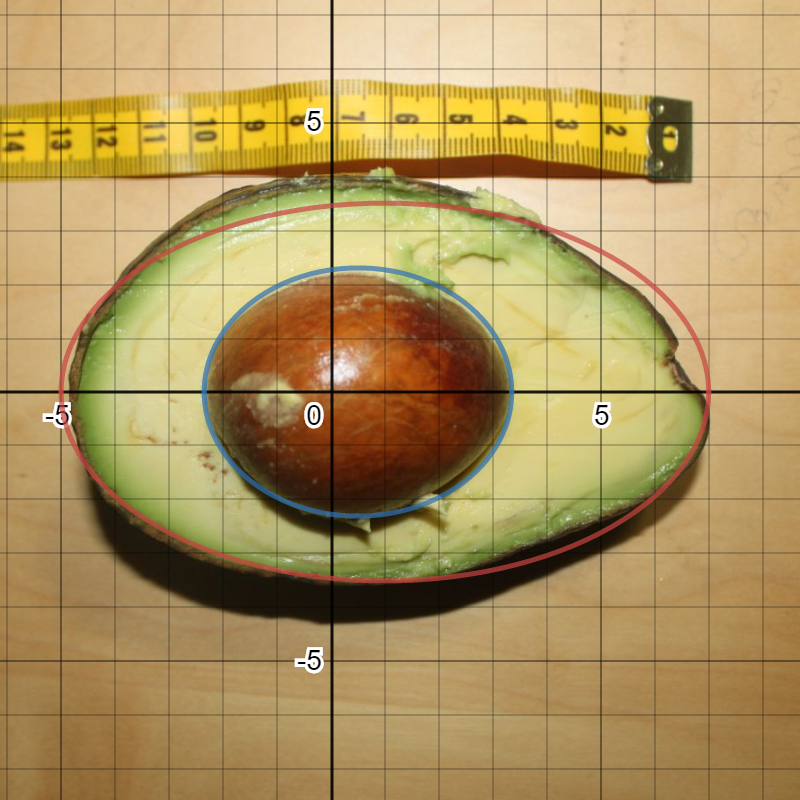
\includegraphics[scale=.2]{avocad.png}
        \caption{\textit{A regular, boring avocado.} Desmos link \href{https://www.desmos.com/calculator/i0kemx2ihg}{\textcolor{blue}{here}}}
    \end{center}
\end{figure}
\section{Solution}
Our first goal is to find the volume of flesh ignoring pit, then subtract the volume of the pit.
\begin{align}
    \intertext{\sout{First, calculate the total volume of avocado needed to survive $1.1$ years}}
    13\frac{cm^3}{.1\:years}\cdot 11\:.1\:years                                   & = \boxed{143\:cm^3}
    \intertext{Then, consider the area of a semicircle, in terms of $radius$, to use in calculating the pit and flesh volume}
    A(r)                                                                          & =\frac{\pi r^2}{2}
    \intertext{Let's put it in terms of $base$}
    r                                                                             & =\frac{1}{2}b                                                                                                                                                    \\
    r^2                                                                           & = \frac{1}{4}b^2                                                                                                                                                 \\
    A(b)                                                                          & = \frac{\pi}{8}b^2
    \intertext{To calculate the flesh volume, we must first find the ellipse volume and subtract from pit volume. To caclulate pseudoflesh volume, first put the ellipse equation in terms of $x$, as the cross-sections are perpendicular to the $x-axis$}
    \frac{\left(x-1\right)^{2}}{6^{2}}+\frac{y^{2}}{3.5^{2}}                      & =1                                                                                                                                                               \\
    \frac{y^{2}}{3.5^{2}}                                                         & =1-\frac{\left(x-1\right)^{2}}{6^{2}}                                                                                                                            \\
    y^{2}                                                                         & =3.5^{2}\cdot\left(1-\frac{\left(x-1\right)^{2}}{6^{2}}\right)                                                                                                   \\
    y                                                                             & =\pm\sqrt{3.5^{2}\cdot\left(1-\frac{\left(x-1\right)^{2}}{6^{2}}\right)}
    \intertext{In this specific case, since the top and bottom of an ellipse are equivalent, we can change the $\pm$ into $2$}
                                                                                  & =2\sqrt{3.5^{2}\cdot\left(1-\frac{\left(x-1\right)^{2}}{6^{2}}\right)}
    \intertext{This can obviously be simplified a bit}
    2\sqrt{3.5^{2}\cdot\left(1-\frac{\left(x-1\right)^{2}}{6^{2}}\right)}         & =\sqrt{49\left(1-\frac{\left(x-1\right)^{2}}{6^2}\right)}
    \intertext{Plug this into our Area function to get area in terms of $x$}
    A(x)                                                                          & =\frac{\pi}{8}(\sqrt{49\left(1-\frac{\left(x-1\right)^{2}}{6^2}\right)})^2                                                                                       \\
                                                                                  & =\boxed{\frac{49\pi}{8}\left(1-\frac{\left(x-1\right)^{2}}{6^2}\right)}
    \intertext{Recall equation for volume}
    \text{3D Volume}                                                              & =\int_{a}^{b}A\left(x\right)dx
    \intertext{To get $a$ and $b$ bounds for the integral, find the $a_1$ value for the ellipse, and account for $h$ values of the ellipse}
    a_1                                                                           & =6                                                                                                                                                               \\
    h                                                                             & =1                                                                                                                                                               \\
    a                                                                             & = -6 + 1                                                                                                                                                         \\
                                                                                  & = \boxed{-5}                                                                                                                                                     \\
    b                                                                             & = 6+1                                                                                                                                                            \\
                                                                                  & = \boxed{7}
    \intertext{Now plugin $A(x)$ and $a$ and $b$ and integrate}
    \int_{a}^{b}A\left(x\right)dx                                                 & =\int_{-5}^{7}\frac{49\pi}{8}\left(1-\frac{\left(x-1\right)^{2}}{6^2}\right)dx                                                                                   \\
                                                                                  & =\frac{49\pi}{8}\int_{-5}^{7}\left(1-\frac{\left(x-1\right)^{2}}{6^2}\right)dx
    \intertext{Why not do some $u-sub$?}
    u                                                                             & = x-1                                                                                                                                                            \\
    du                                                                            & = dx                                                                                                                                                             \\
    (7)-1                                                                         & = 6                                                                                                                                                              \\
    (-5)-1                                                                        & = -6
    \intertext{Substitute}
    \frac{49\pi}{8}\int_{-5}^{7}\left(1-\frac{\left(x-1\right)^{2}}{6^2}\right)dx & =\frac{49\pi}{8}\int_{-6}^{6}\left(1-\frac{\left(u\right)^{2}}{6^2}\right)du
    \intertext{Now, because the left and right sides of an ellipse are equivalent, we can actually take the $-6$ out and factor out a $2$}
                                                                                  & =\frac{49\pi}{4}\int_{0}^{6}\left(1-\frac{u^{2}}{6^{2}}\right)du                                                                                                 \\
                                                                                  & =\frac{49\pi}{4}(u-\frac{u^3}{3\cdot 6^2}\Big|_{0}^{6})                                                                                                          \\
                                                                                  & =\frac{49\pi}{4}\left(\left(6\right)-\frac{\left(6\right)^{3}}{3\cdot6^{2}}-\left(-\left(0\right)-\frac{-\left(0\right)^{3}}{3\cdot6^{2}}\right)\right)          \\
                                                                                  & =\frac{49\pi}{4}\left(6-\frac{6}{3}\right)                                                                                                                       \\
                                                                                  & =\frac{49\pi}{4}\left(6-2\right)                                                                                                                                 \\
                                                                                  & =\frac{49\pi}{4}\left(4\right)
    \\
                                                                                  & =\boxed{49\pi}
    \intertext{Now let's work on the avocado seed. First, put equation in terms of $x$}
    \frac{\left(x-.5\right)^{2}}{2.85^{2}}+\frac{y^{2}}{2.3^{2}}                  & =1                                                                                                                                                               \\
    \frac{y^{2}}{2.3^{2}}                                                         & =1-\frac{\left(x-.5\right)^{2}}{2.85^{2}}                                                                                                                        \\
    y^{2}                                                                         & =2.3^{2}\left(1-\frac{\left(x-.5\right)^{2}}{2.85^{2}}\right)                                                                                                    \\
    y                                                                             & =\pm\sqrt{2.3^{2}\cdot\left(1-\frac{\left(x-.5\right)^{2}}{2.85^{2}}\right)}                                                                                     \\
    y                                                                             & =2\sqrt{2.3^{2}\cdot\left(1-\frac{\left(x-.5\right)^{2}}{2.85^{2}}\right)}
    \intertext{Try to simplify}
                                                                                  & =\sqrt{21.16\cdot\left(1-\frac{\left(x-.5\right)^{2}}{8.1225}\right)}
    \intertext{Plugin to the same area function that we used for the avocado flesh earlier}
    A(x)                                                                          & =                                                                        \frac{\pi}{8}(\sqrt{21.16\cdot\left(1-\frac{\left(x-.5\right)^{2}}{8.1225}\right)})^{2} \\
                                                                                  & =\boxed{\frac{21.16\pi}{8}\left(1-\frac{\left(x-.5\right)^{2}}{8.1225}\right)}
    \intertext{Now to find $a$ and $b$, again consider the $a_1$ and $h$ values of the ellipse}
    a_1                                                                           & =2.85                                                                                                                                                            \\
    h                                                                             & =.5                                                                                                                                                              \\
    a                                                                             & =-2.85+.5                                                                                                                                                        \\
                                                                                  & =\boxed{-2.35}                                                                                                                                                   \\
    b                                                                             & =2.85+.5                                                                                                                                                         \\
                                                                                  & =\boxed{3.35}
    \intertext{Now plugin to the equation for volume}
    \int_{a}^{b}A\left(x\right)dx                                                 & =\int_{-2.35}^{3.35}\frac{21.16\pi}{8}\left(1-\frac{\left(x-.5\right)^{2}}{8.1225}\right)dx                                                                      \\
                                                                                  & =\frac{21.16\pi}{8}\int_{-2.35}^{3.35}\left(1-\frac{\left(x-.5\right)^{2}}{8.1225}\right)dx
    \intertext{Let's just FOIL it out this time. I think that this demonstrates how messy the process can be if you don't $u$-sub and break it down into smaller parts.}
                                                                                  & =\frac{21.16\pi}{8}\int_{-2.35}^{3.35}\left(1-\frac{\left(x-.5\right)^{2}}{8.1225}\right)dx                                                                      \\
                                                                                  & =\frac{21.16\pi}{8}\int_{-2.35}^{3.35}\left(1-\frac{\left(x^{2}-x+.25\right)}{8.1225}\right)dx                                                                   \\
                                                                                  & =\frac{21.16\pi}{8}\left(x-\frac{1}{8.1225}\cdot\left(\frac{x^{3}}{3}-\frac{x^{2}}{2}+.25x\right)\right)\Big|_{-2.35}^{3.35}
\end{align}
\begin{equation}
    =\frac{21.16\pi}{8}(3.35-\frac{1}{8.1225}\cdot\left(\frac{3.35^{3}}{3}-\frac{3.35^{2}}{2}+.25\cdot3.35\right)
\end{equation}
\begin{equation}
    +2.25+\frac{1}{8.1225}\cdot\left(\frac{\left(-2.25\right)^{3}}{3}-\frac{\left(-2.25\right)^{2}}{2}+.25\left(-2.25\right)\right))
\end{equation}
\begin{align}
                   & = \frac{21.16\pi}{8}\left(3.79653226634...\right) \\
                   & \approx\boxed{10.04\pi}
    \intertext{Anyways, now we just subtract the pseudoflesh volume by the pit volume}
    49\pi-10.04\pi & = 38.96\pi                                        \\
                   & \approx\boxed{122.40\:cm^3}
    \intertext{\sout{Compare volumes for your answer}}
                   & \boxed{122.40\:cm^3 < 132\:cm^3}
\end{align}
\section{Conclusion}
\sout{Bob should leave the city and start a new country life with his avocado!}
Tell George the volume of the avocado is $122.40\:cm^3$
\end{document}